%% generated by mpce_csweep.py -- do not edit by hand
%% Supplementary: PSO coefficient sweep and bound handling (review round 2, R3 #1); requires booktabs,
%% graphicx and mpce_numbers_csweep.tex

\begin{figure*}[!t]
\centering
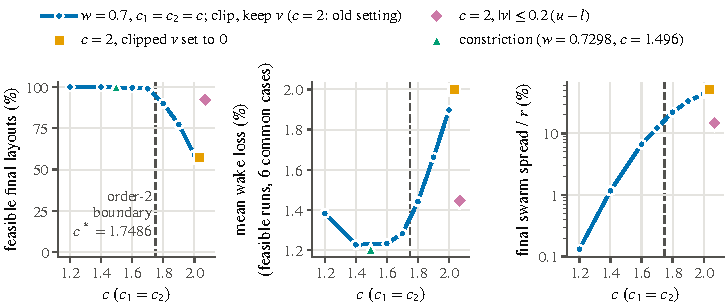
\includegraphics[width=\textwidth]{figures_mpce/csweep.pdf}
\caption{Stand-alone PSO with $w=0.7$ and $c_1=c_2=c$ on the 12 split cases $\times$ 30 seeds (6{,}030 evaluations, random starts; line with circles), the old setting ($c=2$) with two other bound-handling rules (clipped velocity components set to zero; velocity clamping $|v|\le v_{\max}=0.2\,(u-l)$; drawn slightly to the right of $c=2$), and the constriction setting ($w=0.7298$, $c=1.49618$; stored runs of the main comparison, spread not logged). The dashed vertical line is the order-2 stability boundary $c^\ast=12(1-w^2)/(7-5w)=1.7486$ of Proposition~\ref{prop:S-pso-stability} (stagnation, no bounds). Left: feasible final layouts (\% of 360 runs). Middle: mean wake loss of the feasible runs, averaged over the 6 cases in which every setting has at least 15 feasible runs. Right: median final swarm spread (mean over particles of the RMS turbine distance to the global best), relative to the farm radius (log scale). All settings start from the same seeded initial swarm. Values: Table~\ref{tab:S-csweep}.}
\label{fig:S-csweep}
\end{figure*}

\begin{table*}[!t]
\centering
\caption{PSO coefficient sweep and bound handling (12 split cases $\times$ 30 seeds, 6{,}030 evaluations, random starts). Feasible: final layouts feasible (\% of 360 runs); $N\ge10$: the same for the 180 runs with $N=10, 12, 15$; qualified: cases with at least 15 of 30 feasible runs; $L$: mean wake loss (\%) of the feasible runs, averaged over the 6 cases in which every setting is qualified; $L_{12}$: the same over all 12 cases (only for settings qualified in all 12); rank: average rank over the 12 cases among the ten settings (feasibility-aware rule of the main comparison: settings with fewer than 15 feasible runs rank below all qualified ones); spread: median final swarm spread relative to the radius (\%); clipped: coordinates leaving the box per iteration (\%, iterations 1--200); feasible evals: particle evaluations with a feasible layout in iterations 101--200 (\%). The row $c=2.0$ reproduces the stored runs of the old setting bit for bit; the constriction row is the stored PSO data of the main comparison (dynamics not logged). Order-2: whether $(w,c)$ satisfies the order-2 condition of Proposition~\ref{prop:S-pso-stability} ($c<\NSBoundC$ at $w=0.7$), which assumes no velocity clamping. For every setting and seed, the final layout is feasible in Data Set~I if and only if it is feasible in Data Set~II (same geometry; the penalty dominates while a layout is infeasible), so the feasibility columns rest on 6 geometries $\times$ 30 seeds.}
\label{tab:S-csweep}
\scriptsize\setlength{\tabcolsep}{3.5pt}
\resizebox{\ifdim\width>\textwidth\textwidth\else\width\fi}{!}{%
\begin{tabular}{cclcccccccccc}
\toprule
$w$ & $c$ & Bound handling & Order-2 & Feasible (\%) & $N\ge10$ (\%) & Qualified & $L$ (\%) & $L_{12}$ (\%) & Rank & Spread (\%) & Clipped (\%) & Feas.\ evals (\%) \\
\midrule
0.7 & 1.2 & clip, keep $v$ & yes & 100.0 & 100.0 & 12 & 1.38 & 3.05 & 5.42 & 0.1 & 0.5 & 80.4 \\
0.7 & 1.4 & clip, keep $v$ & yes & 100.0 & 100.0 & 12 & 1.23 & 2.77 & 2.50 & 1.2 & 0.9 & 69.9 \\
0.7 & 1.6 & clip, keep $v$ & yes & 99.4 & 99.2 & 12 & 1.23 & 2.77 & 2.33 & 6.6 & 1.9 & 41.5 \\
0.7 & 1.7 & clip, keep $v$ & yes & 98.9 & 98.3 & 12 & 1.28 & 2.93 & 3.58 & 12.2 & 2.9 & 25.4 \\
0.7 & 1.8 & clip, keep $v$ & no & 90.0 & 85.0 & 12 & 1.44 & 3.37 & 6.17 & 22.1 & 4.3 & 13.1 \\
0.7 & 1.9 & clip, keep $v$ & no & 77.2 & 65.8 & 10 & 1.66 & -- & 7.83 & 33.4 & 6.3 & 5.6 \\
0.7 & 2.0 & clip, keep $v$ & no & 58.9 & 38.3 & 6 & 1.90 & -- & 9.17 & 43.6 & 8.7 & 2.6 \\
\midrule
0.7 & 2.0 & clip, $v\gets0$ & no & 57.2 & 35.8 & 6 & 2.00 & -- & 9.83 & 50.8 & 8.8 & 2.5 \\
0.7 & 2.0 & $|v|\le v_{\max}$, clip & no & 92.2 & 88.3 & 12 & 1.45 & 3.42 & 6.42 & 14.7 & 1.6 & 11.8 \\
0.7298 & 1.496 & clip, keep $v$ & yes & 100.0 & 100.0 & 12 & 1.20 & 2.69 & 1.75 & -- & -- & -- \\
\bottomrule
\end{tabular}}
\end{table*}
